\chapter{The detection problem}
In the previous chapter, we have presented the physical background of ionograms. We have also shown the four major features that can be detected in them. In this part we try to make a transition to the technical point of view. Firstly we define the problem in the context of computer vision. Secondly we describe the data formats and finally we present the current situation about feature detection in ionograms and an analysis on how the problem could be solved.

\section{Definitions}
Now we are to seek for definitions of the basic terms used throughout the rest of this work. In order to precisely define the detection problem, we need to know the definitions of what a ionogram or its feature is. We also specify what attributes should a detection result have. Finally, we introduce some measures of quality of the detection along with formulating the problem.

\subsection{Definition of ionogram}
As stated in section \ref{sec:ionograms}, a ionogram consists of electric field density measured at 160~frequencies and within 80~consequent time steps. Thus, we can treat a ionogram as a real-valued image (or a two-dimensional array) of dimension 160x80. The range of values at each pixel is \n{E-24} to \n[V^2m^{-2}Hz^{-1}]{E-10}\footnote{We haven't found an authoritative source for this information, but instead we deduced it from a large set of ionograms.}. However, it is obvious from the sample renderings in \citep{FTP} that values lower than \n{E-17} are considered to be background, so we can treat them as zeros. The horizontal indices are interpreted as the sounding frequency and they come from the range \n{0.1} -- \n[MHz]{5.5}. The mapping from indices to frequencies is nonuniform and may differ for individual ionograms (it depends on the used frequency table; but a single table is preferred in most of the data). Every ionogram carries information about this mapping with it. On the other hand, the vertical indices map always to the same uniformly distributed values. They start at \n[{\upmu}s]{162.5} and go up to \n[ms]{7.32} using steps of height \n[{\upmu}s]{91.4} (assuming the lowest value to be at top).

As we are going to detect repetitious features, the ionogram with unevenly distributed frequency assignment would be impractical. To overcome this, we define our notion of ``evenly sampled ionogram''. To get an evenly sampled ionogram from a normal ionogram, we linearize the frequency axis and then interpolate the ``holes'' in the image:

\begin{itemize}
  \item We first extend each frequency column of the unevenly sampled ionogram by mapping the columns to a linear axis. The pixel width of the linear axis should be at least the frequency range (\n[MHz]{5.4}) divided by the frequency width of the narrowest column (in order to allow every new column to have its width at least \n[px]{1}). We also stretch rows by the same amount to preserve aspect ratio. In practice we scale the ionograms so that the narrowest column has width \n[px]{2} to get a finer result. The size of such ionograms is then \n{1012}x\n[px]{506}. See Fig. \ref{fig:even_uneven_iono} for illustration.
  \item Next we interpolate the new columns using linear interpolation. Suppose column $i$ from the unevenly sampled ionogram stretched to columns $j$\ldots$j+k$ in the evenly sampled one. The values at column $j$ are copied from $i$ and for every column $c\in<j+1; j+k>$ its value is $$v[c] = v[j]*(1-\frac{c-j}{k}) + v[j+k+1]*\frac{c-j}{k}$$ where $v[c]$ denotes the vector of values at column $c$, $j$ and $j+k+1$ are the remapped columns corresponding to two originally neighboring pixels. In fact we just linearly interpolate the ``holes'' using the two nearest values from the original image. Fig. \ref{fig:even_uneven_iono} gives a visualization of this step. 
  \item Then we perform the same interpolation vertically to fill missing values in columns. The final evenly sampled ionogram can be found in Fig. \ref{fig:even_uneven_iono}.
\end{itemize}

This interpolation of course does not add any new information to the image, but it allows us to work on an image with both axes in uniform linear scale. We have chosen this kind of interpolation because it is the one used in the referential renderings available at \citep{FTP}. We have simplified it by not caring about the values near edges, because they have insignificant impact on the results of detection. Nonetheless, any other kind of interpolation of missing pixels can be used as long as it preserves the values corresponding to the ``original pixels'' (e.g. plain pixel enlargement with copying the values instead of interpolating them).

\begin{figure}[H]
	\centering
	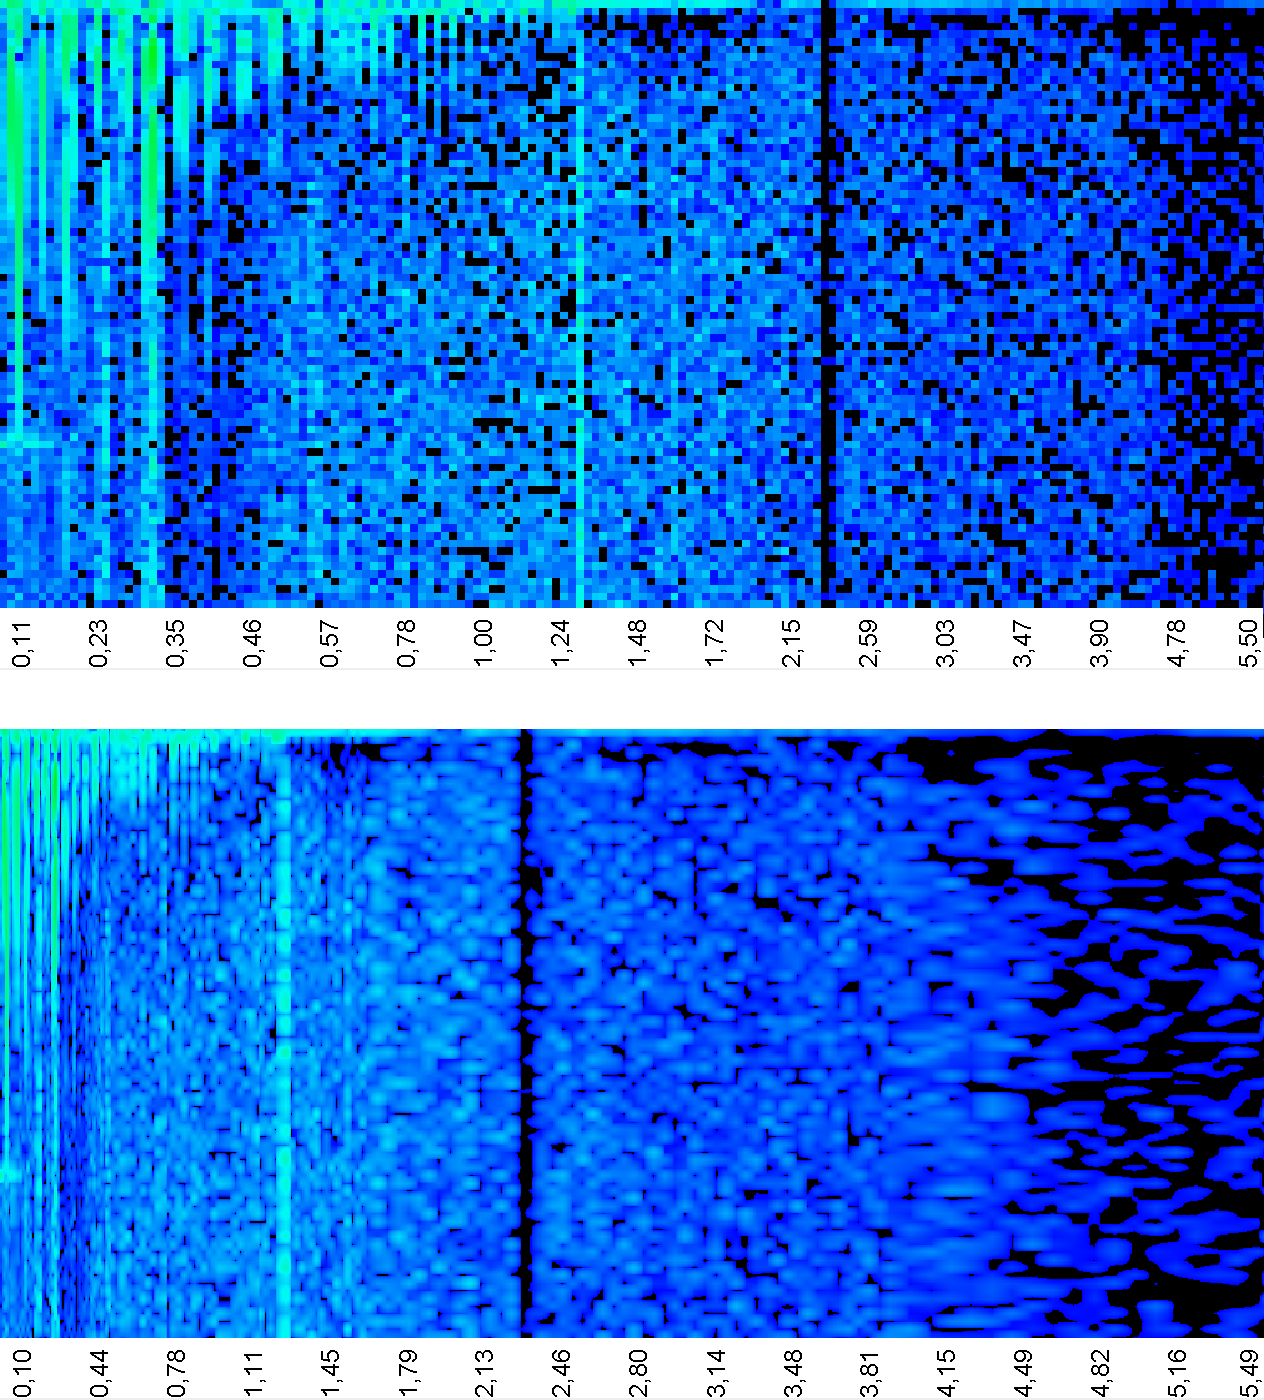
\includegraphics[width=140mm]{images/even_and_uneven_ionogram.png}
	\caption{a) A part of the original unevenly sampled ionogram. b) The original ionogram mapped to a linear horizontal axis. Every original pixel is only mapped to one pixel in this image, the other pixels remain black. Here it is noticeable that values on the left are more dense than these on the right. This is due to the quasi-logarithmic distribution of sounding frequencies. c) Our evenly sampled ionogram after horizontal interpolation. d) Our evenly sampled ionogram after vertical interpolation. Data from orbit 3874, frame 0 \citep{FTP}.}
	\label{fig:even_uneven_iono}
\end{figure}

\subsection{Specification of the features to detect}
We have listed four features of interest - ionospheric echoes (IE), ground echoes (GE), electron plasma oscillation harmonics (EPOH) and electron cyclotron harmonics (ECH) (in section \ref{ssec:oblique} we have already stated we omit oblique ionospheric echoes). We detect them based on the fact that they correspond to areas with significantly higher ionogram values than the background. However, ionograms are often very noisy, so it would be difficult (if not impossible) to define a single absolute threshold for telling whether a pixel belongs to a feature or not. 

For verification purposes we manually tagged \n{115495} ionograms from \n{1014} orbits during year 2007. In most of these ionograms we measured manually the horizontal repeat period (corresponding to EPOH) and marked the ionospheric echoes. If no horizontal repetition period was present, we recorded that fact, too. Although being done manually and thus each feature being assessed subjectively, we deduced our rules for distinguishing interesting lines (which are either a feature or a part of a feature). Such line is several pixels wide (cca. 3--\n[px]{20}) and at least that much pixels long (assuming the ionogram has dimension \n{1012}x\n[px]{506}). Values on its skeleton (center line) are at least 10 times higher than those at its border. A line is also allowed to contain ``gaps'', but no more than a third of the line's length in sum. Moreover, every line should contain a value higher than cca. \n{5E-15} (but not all points with higher values belong to a feature). Such definition looks, however, vague. So we propose additional specific constraints implying from the features we try to detect in our experiments. 

An EPOH or ECH line must be almost straight and must go in exactly vertical or horizontal direction. In addition, one of its ends has to be near the top or left edge of the ionogram (no more than \n[px]{5}). ECH lines usually do not extend to frequencies above \n[MHz]{2.5}. A GE line follows approximately horizontal direction and does not have to be straight (due to terrain unevenness and the cusp; but mostly it is). It is placed in the delay time (or apparent height) corresponding to the height of the spacecraft over surface (that can be computed) which greatly helps in its detection. Finally, an IE line has also to be almost horizontal, but it may be substantially curved. It has to appear over the GE (if present).

Our statistical tests we conducted\footnote{The application used for these tests is present on the attached CD in folder \texttt{programs/statistics} along with the data. See \nameref{sec:running} for information on how to run it.} on the data from year 2007 show that \n[\%]{99.5} ionograms with some features have their mean value greater than \n{2.45216E-16}. Ionograms devoid of features have, of course, their mean values even lower than this value (in \n[\%]{21.5} of cases). So we decided this value to be a threshold for telling a ionogram does not contain any features and we will not process it further. We did not choose lower reliability level because we do not want to throw away ionograms with some data present.

We also computed other statistical properties of ionograms that could help us better distinguish the features. We expected the maximum values in ionograms to be a reliable distinguishing mark, and standard deviations, too. As shown in Fig. \ref{fig:data_stats}, neither maxima nor standard deviations show significant differences between the data sets with features and without them. So they are not usable for distinguishing between the two data sets. We also made distributions of rather high values (over \n{E-12}) in relation to whether they are a part of a feature or not. The results showed almost identical distributions, but that can be due to the difficulty of reverse task. E.g. if we save just the period of an EPOH, it is not easily said if a data point belongs to this feature (we try to fit it on whole multiplies of the period, but we do not know the widths of the particular lines). 

\begin{figure}
	\centering
	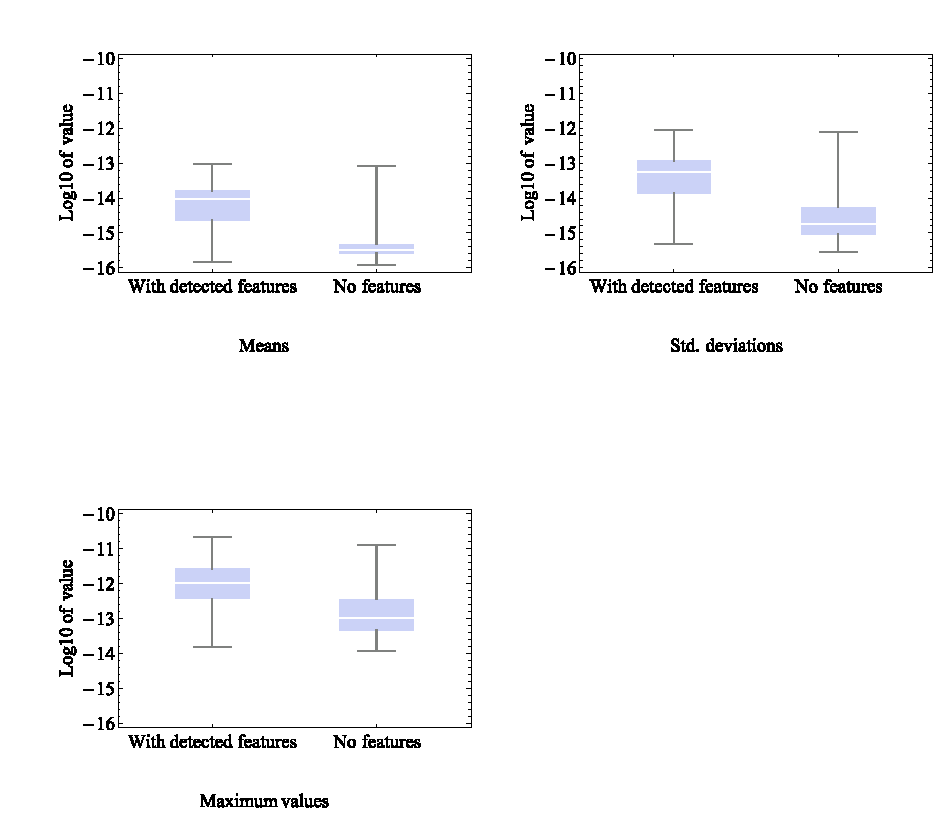
\includegraphics[width=140mm]{images/data_stats.pdf}
	\caption{The distribution of means (top left), standard deviations (top right) and maximum values (bottom left) of individual ionograms from year 2007. The box plots show values for ionograms with features and without features separately. Data from \citep{FTP}.}
	\label{fig:data_stats}
\end{figure}

\subsection{Specification of the detection results}
Having an idea about how to recognize a feature, we can finally define the form of the results of our detection. Here it is important to declare we are not interested in the graphical shapes, rather we want to get results directly applicable in the physical models described in section \ref{sec:ionograms}. 

From section \ref{ssec:epoh} follows that to get the local electron plasma frequency from EPOH, it is sufficient to have the period of the harmonics. It is not important how long or wide the harmonic echoes are, only the period of repetition. We  denote this period as ``hPeriod'' (horizontal period) and measure it in MHz\footnote{It may seem a little confusing to show a period in MHz, but it should rather be looked at as the difference of two sounding frequencies producing echoes.}.

Similarly, as noted in section \ref{ssec:cyclotronEchoes}, to get the local electron cyclotron frequency from ECH, it is also sufficient to know the repetition period. We term this period as ``vPeriod'' (vertical period) and measure it in milliseconds. 

The situation for ionospheric and ground echoes is quite the same. What we need is the time delay when the sounding wave first returned back with high intensity to derive height over ionosphere border or ground. We are also interested in the rightmost point of IE and leftmost point of GE (the cusp described in section \ref{ssec:ie}) to be able to read off the maximal electron plasma frequency f$_p$(max). The left end of the IE should start at the local electron plasma frequency, but it is read more reliably from EPOH. In conclusion, for both IE and GE we need to save the positions of all points on the top border of these echoes. We save it in ionogram coordinates, which are sounding frequency in MHz and delay time in milliseconds.

\subsection{Definition of the detection problem}
Now we have all definitions needed to state the ``detection problem''. Given a ionogram $\mathcal{I}$, find a (possibly empty) set of detection results $\mathcal{R}$ corresponding to all features occurring in $\mathcal{I}$. Simultaneously minimize the number of false positives (found features not existing in fact) and false negatives (undetected existing features) and also minimize distance of the detection result values to the values of real features. As it is a multivariate optimization problem, we do not convert it to univariate optimization by specifying weights, we assess all three aspects separately.

Unfortunately, we do not have an oraculum divining the values of real features. Instead we have to replace it with the manually acquired data, which is the best approximation of the oraculum we can get. The drawbacks are, however, that the manually created data are not perfect, so the tested algorithms can seem to be better than in fact and vice versa simply due to the inaccuracy of the validation set. Until there are alternative ways to measure the observed values, manual verification is the best we have.

So we can reformulate the problem as finding detection results with minimum error on the verification set and with good generalization on other ionograms.

We can also generalize our whole problem (calling it the ``generalized detection problem'') from ionograms to general images. Given an image $\mathcal{I}$ and a set of rules $\mathcal{S}$ describing the features to be found in $\mathcal{I}$, return the (possibly empty) set of detection results $\mathcal{R}$ containing all features described by $\mathcal{S}$ present in $\mathcal{I}$. To measure the quality, a verification set of pairs ($\mathcal{I}$, $\mathcal{R}$) should be provided. As a simplification we assume that $\mathcal{S}$ contains only features that can be described using curves or curve structures (like repeating lines).

Roughly approximating, we can say the problem is a vectorization problem with known parametric expressions for some of the features in the image. As we show further, many vectorization techniques can be used for solving our problem.

\section{Data formats}
In this short section we describe our used input and output data formats and also the source for obtaining ionograms. This is the last step to do before we get to the analysis of our problem. 

\subsection{Data source}
All data captured by the MARSIS instrument (and the others too) are stored in the Planetary Science Archive (PSA) run by ESA. It is located at WWW: \url{http://www.rssd.esa.int/index.php?project=PSA}. We access it using anonymous FTP access and the Active Ionospheric Sounding (AIS) data are stored at \url{ftp://psa.esac.esa.int/pub/mirror/MARS-EXPRESS/MARSIS/MEX-M-MARSIS-3-RDR-AIS-EXT1-V1.0/DATA/ACTIVE\_IONOSPHERIC\_SOUNDER/}. There are subfolders for every 10 orbits in the archive (named e.g. \texttt{RDR193X} for orbits 1930--1939). In these subfolders there are files named \texttt{FRM\_AIS\_RDR\_(orbit number).LBL} which contain metadata about the orbit. Each such metadata file references a data file named \texttt{FRM\_AIS\_RDR\_(orbit number).DAT} containing the sounding data.

We remark that for some orbits there are no AIS data available when MARSIS was not instructed to operate. E.g. from the cca. \n{1300} orbits in year 2007 we processed manually there are \n{1014} orbit data files.

\subsection{Input files format}
The metadata (.LBL) files are text files formatted according to the Planetary Data System (PDS) v3 format defined in \citep{JPL2009}. Although the format can be quite complex, to parse the metadata we are interested in, just a simple line-by-line text parser is sufficient.

The orbit data (.DAT) are stored according to the binary format specified in Attachment \ref{att:format}. Every orbit data file contains frames which can be interpreted as individual ionograms. There are 30 -- 400 frames per orbit depending on the observation conditions and other possibly interfering MEX operations. 

Every frame further consists of 160 columns records each of 80 elements. Every column record (corresponding to one sounding pulse) carries information about the exact time the sounding started, the sounding frequency and much more parameters we are not interested in.

We implemented a reader for the .LBL and .DAT files that re\-turns the corresponding Java objects. It is located on the attached CD in folder \texttt{programs/AIS-Data-Reader}, namely classes \texttt{Ionogram} and \texttt{AISLBLProductReader}. See \nameref{sec:running} for information on how to run it.

\subsection{Output files format}
To be consistent with the input files, we have decided to use 1~result file per orbit, too. We name it \texttt{TRACE\_(orbit number).XML} and place it to the same folder as the source .DAT file. However, contrary to the input data files, we have decided to store the results in text files using XML (XML Markup Language) structure. There are two main reasons. The first is the most important one -- the result files are small in comparison to the data files, so we can afford some inefficiency introduced by text encoding. The second reason is straightforward -- XML~files are easy to read even for humans and parsing them is a simple task.

The structure of the file is shown in Attachment \ref{att:result} using the XML Schema language. The main element represents the whole orbit, and there are elements for every frame from the input file. These elements contain the values we detect, namely in elements \texttt{<hPeriod>}, \texttt{<vPeriod>}, \texttt{<ionospheretrace>} and \texttt{<groundtrace>}. If no EPOH or ECH is present, the corresponding values are set to \n{0.0} to indicate absence of these features.

We provide a set of Java classes able to convert between the output XML and Java objects. These classes can be found on the attached CD in folders \texttt{programs/AIS-Result} and \texttt{programs/AIS-Result-Converter}. The classes make use of the widely used Java And XML Bindings v2 (JAXB2) de/serialization framework \citep{Java.net2013}. See \nameref{sec:running} for information on how to run it.

\section{Automated detection}
This section mentions the current status of solving the problem. Then we follow with an analysis of the problem and explore the ways possibly leading to an automated detection solution. These open ideas and propositions conclude this chapter.

\subsection{Current ways of solving the problem}  

\begin{figure}
	\centering
	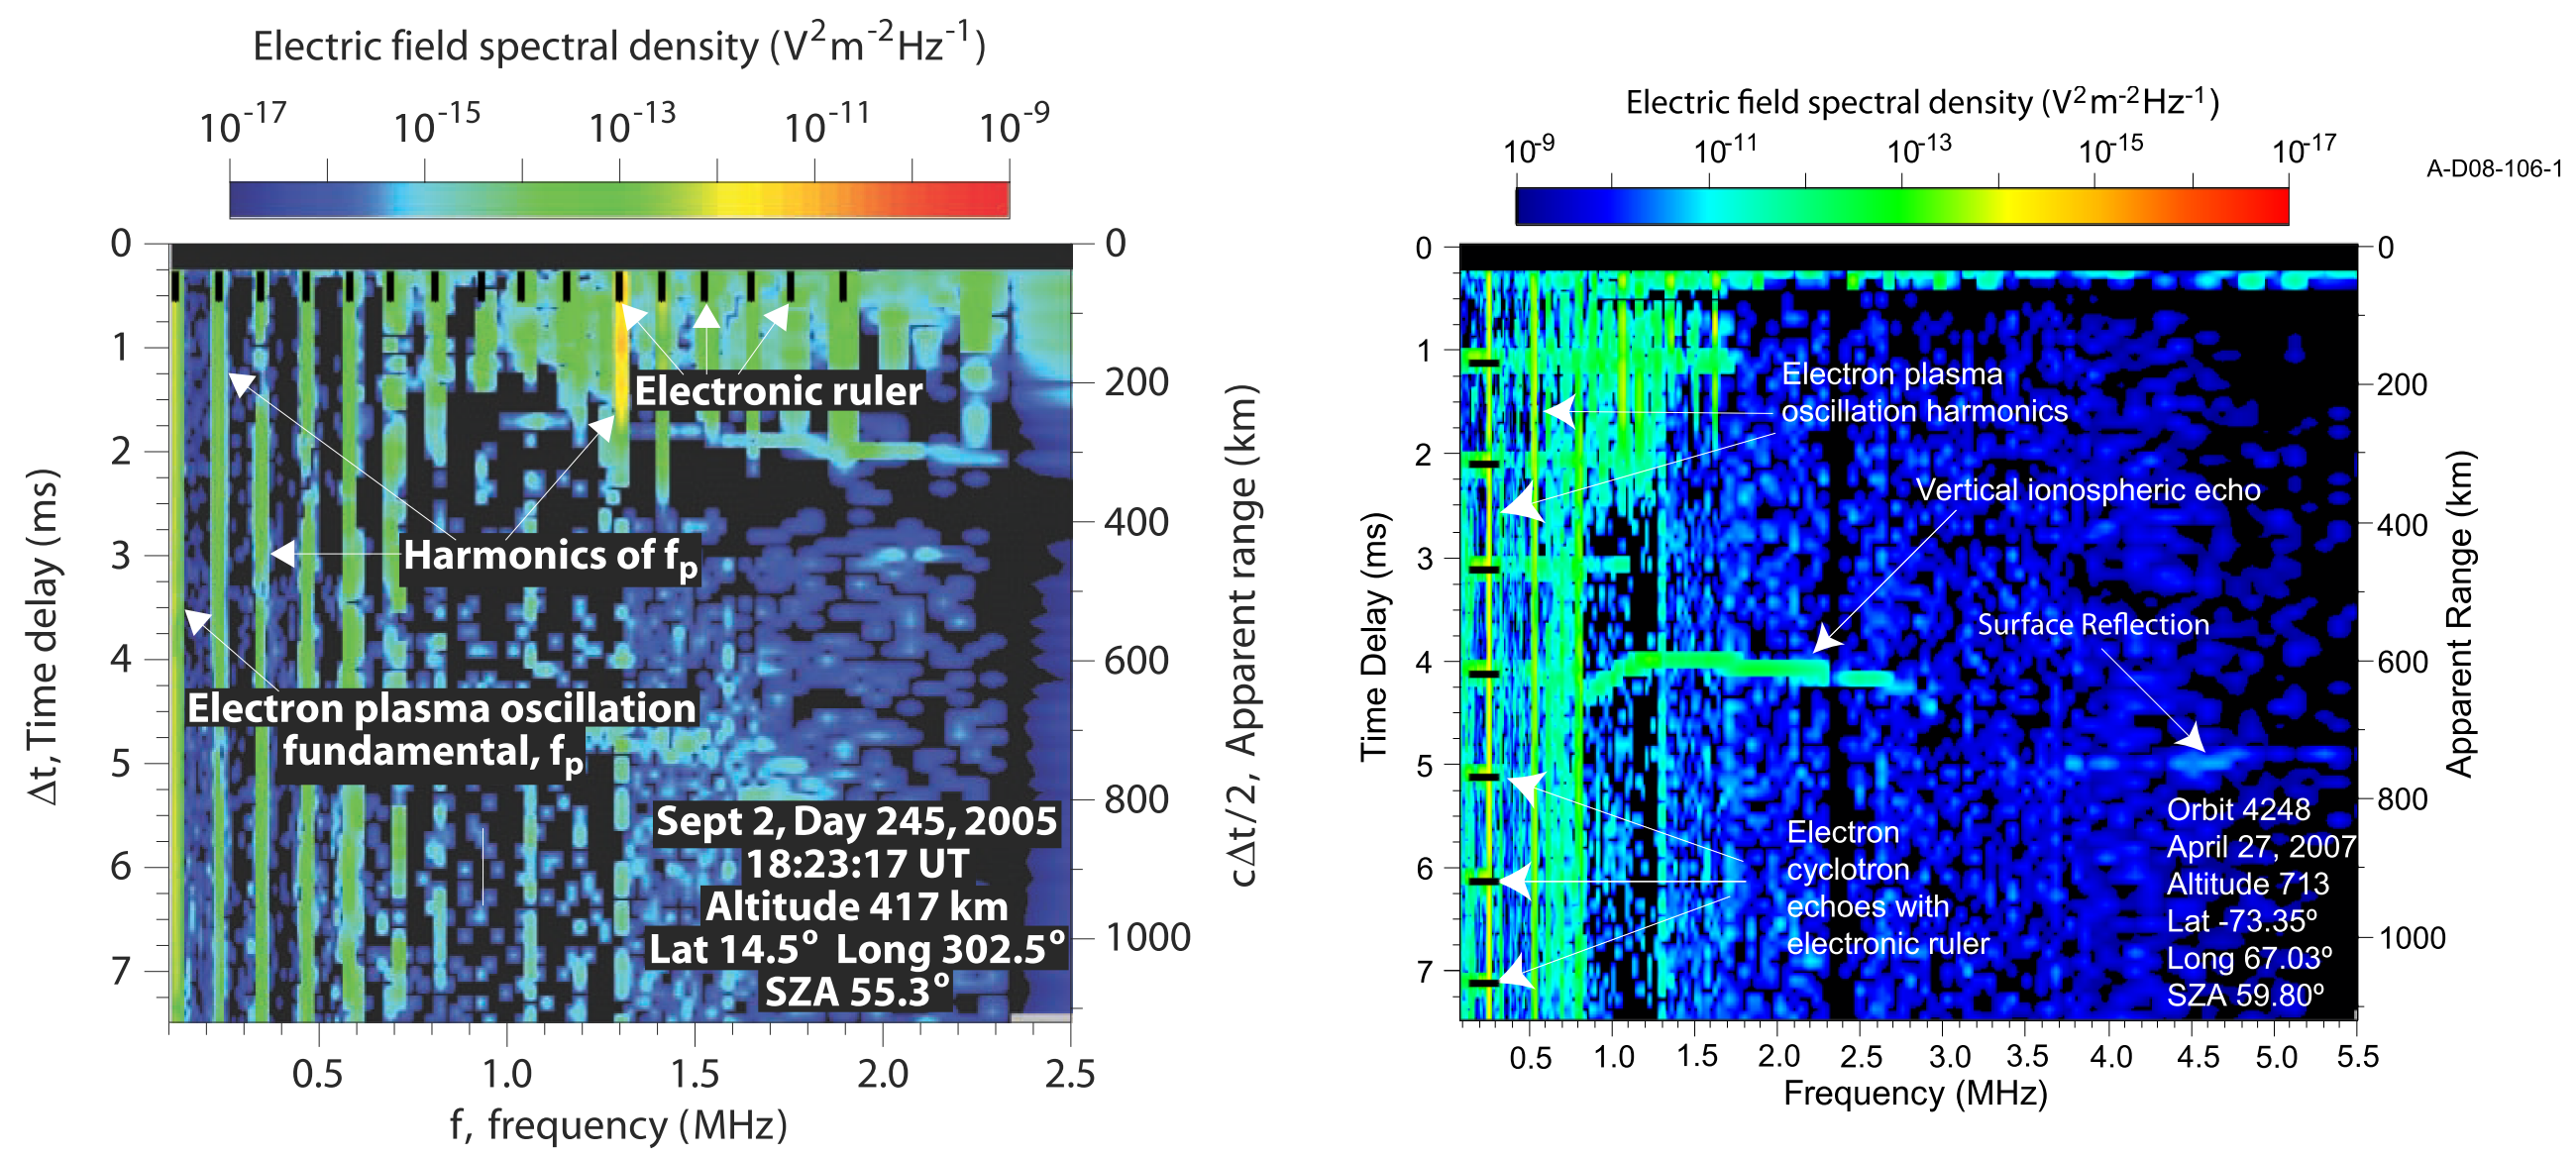
\includegraphics[width=140mm]{images/rulers.png}
	\caption{Previews from the software for manual measurements of horizontal and vertical spacings. In the left image there are horizontally placed black tick marks near the top border for measuring EPOH \citep{Duru2008}. The right image shows vertically repeating black tick marks near the left edge which serve for measuring ECH period \citep{Akalin2010}.}
	\label{fig:rulers}
\end{figure}

As far as we know there is currently no fully automated software solving the formulated problem. All the measurements are performed manually by visual tools. We think it is due to the requirement on high precision of the detected values. The Department of Physics and Astronomy, University of Iowa, developed a software called ``MARSIS Ionogram Survey'' for the manual recording of visual measurements. However, using the software requires authorization from the department.

Nevertheless, some screenshots illustrating the basic idea were published \citep{Duru2008, Akalin2010}. We provide them in Fig. \ref{fig:rulers}. As can be seen in both images, there are evenly spaced black tick marks laid over a ionogram. The period between these tick marks is easily adjusted by moving the computer's mouse. The operator then displays a ionogram and matches the tick marks against the repetition period he recognizes in the ionogram. This way the vertical and horizontal period can be easily measured -- only a \n[\%]{1} error in the detected frequency can be reached \citep[p.~2]{Duru2008}.

Digitization of the IEs and GEs is done by selecting the top edge using mouse and a tool that draws piecewise-straight horizontal lines. The result then may look like stairs with unevenly long steps, which is what the top edge of ionograms most often looks like. These lines are then sampled using the original sampling of the ionogram and saved one point per sounding frequency.

The absence of an automated tool for this work was the main reason for choosing this topic of our thesis. Computer vision provides plenty methods for similar tasks. We discuss them in the next section.

\subsection{Proposed solutions}
To start exploring the fields of computer vision that offer useful algorithms for our problem, we first need to narrow down the classification of this problem. It is clear that we do not have to look outside the computer vision field, because that is what our task is about -- automatically doing something that is relatively easy for human sight. 

At first glance our task of automated detection may resemble pattern recognition (PR). There is, however, a problem with not having the patterns to match. What we have is a parametric expression for the features. And the general pattern recognition methods work only with a limited, final and constant set of patterns. Fortunately, looking at the problem closer yields a way to use these methods at least for the repeating lines. If we take a PR method invariant to pattern scale, we can use repeating lines with unit period as the pattern and let the algorithm match it. If the algorithm allows getting the scale of the pattern, the real repetition period is easily found. Due to the relatively small resolution of the non-uniform ionograms (which are sufficient for finding IEs and GEs) we would be also able to generate a list of shapes an IE or GE can have. Using this list as the set of patterns could bring us some results (but there are imminent cases of false positive detections). 

The second field we consider helpful to solve similar tasks is vectorization. Converting bitmaps to vectors is exactly what our problem needs. A lot of work in this field is, however, done in vectorization of technical drawings which is based on assumptions not applicable to our problem. For example the technical drawings have relatively low level of noise (which ionograms do not have) and they have thin, accurate lines (most often drawn by hand with a ruler). The lines in ionograms are most fuzzy and noisy. Thus, edge detection commonly used in these algorithms does not give useful results applied to ionograms. But these algorithms are not worthless. If we manage to perform a thinning or skeletonization algorithm (described further) on ionograms, suddenly the fuzzy lines could become thin and accurate and thus suitable for use with these algorithms. Noise reduction could also help.

Using a specific property of EPOHs and ECHs we could reach good results using a very simple technique. If we compute the row or column sums of the ionogram values (the electric field density), we get a profile with high peaks corresponding exactly to the repeating lines. The other two features (IEs and GEs) do not affect these profiles much (because they are relatively smaller compared to EPOHs and ECHs; only IEs in ECHs may cause problems), as well as noise does not. Having the peaks detected it is needed to estimate the period (since the peaks may be slightly displaced). We propose several methods for such detection: computing a periodogram of the peaks distribution (see Sec. \ref{ssec:periodogram} for definition), fitting a sine wave to the peaks or taking an average period. It is also desirable to use the ``height'' of the peaks as weights for the mentioned methods (since the higher the peak is, the higher is the probability it really belongs to the desired line and not to noise or other features). With the knowledge of the height above surface, row sums can also be used to decide if GE is present and to find its left end. This is because ECHs usually do not extend to the right half of ionogram where GEs usually appear, so we can take only the right half of the image. It is possible to proceed without the height information, too, but the task simplifies if we use it. The last feature, IEs, could also be detected using row and column sums, but it would need cancellation of all three preceding features from the image, which does not seem feasible. Without the ECH lines cancelled out the echo would not be reliably distinguishable from the harmonics line -- in fact, it can even merge with them in the row sums.

We also consider evolutionary algorithms (EAs) as a method worth trying. In EAs, we initialize a population of individuals (representing the detection results) randomly. Then we let them recombine and mutate using some defined operators. We periodically select the best of them (according to a defined fitness function) to survive to the ``next round'', let them reproduce and start the whole process over. The algorithm ends when the individuals converge to an acceptable solution. \pdfcomment{Jeste dohledam citace, az o tom budu psat kapitolu} It is apparent what an individual should look like -- a vector with values for hPeriod, vPeriod and some more points defining the IE and GE. If we manage to design good recombination and mutation operators, as well as fitness, the results could be interesting.

We have just presented the areas of interest, in which we perform our research. For every area we propose several algorithms, describe them and test on the current data from year 2007. The subsequent chapters are dedicated each to one area.